\section{�berblick}
\subsection{Analyse Datenbank BVG}
Die BVG nutzt f�r die Persistierung der Daten, inklusive der Prozessdaten, ein Datenbanksystem der Firma Oracle. Es werden bei der BVG zwischen zwei verschiedenen Systemen unterschieden. Zum einen gibt es die sogenannte SC05 Schnittstelle. Diese enth�lt Prozessdaten der aktuellen Betriebslage. Dazu z�hlen unter anderen Positionen von Bussen und deren Versp�tung. (vgl.: "`Die Prozessdatenschnittstelle (SC05) spiegelt die aktuelle Situation im RBL wider."') % TODO
 Zum anderen gibt es die SC51 Datenbank, entwickelt von der Firma Alcatel. Diese Schnittstelle enth�lt unterschiedlichste Daten f�r Durchf�hrung des �ffentlichen Nahverkehrs der BVG. Darunter fallen Informationen zu Linien (Bus und Bahn), Informationen �ber deren Routen mittels geografischer Koordinaten und vieles mehr.
 F�r die Analyse dieser relationaler Datenbanken waren jeweils deren Dokumentationen und ein Dump zur Verf�gung.
 
 Der erste Schritt der Analyse bestand darin, die Dumps der Oracle Datenbank zu importieren, um anschlie�end Zugriff auf die Tabellen und deren Daten zu erlangen. F�r den Import viel die Entscheidung f�r das Tool "`OraDump to MySQL"'. % TODO https://www.convert-in.com/ord2sql.htm
 Mit diesem Tool ist es m�glich ein Oracle Datenbank Dump in eine MySQL Datenbank zu importieren. Vorteil dieser Methode ist, das auf bestehende Kenntnisse mit dem Umgang von MySQL zur�ckgegriffen werden kann. Im folgenden wurde mittels der Schnittstellen Dokumentation die Struktur der Datenbank analysiert. Im Fokus dieser Analyse stehen die Routen Information aus der SC51 und die Positionsdaten der Fahrzeuge aus der SC05 Schnittstelle. Bei der Analyse haben sich folgende Datenbanktabellen als Wertvoll gezeigt. 
 
Die Tabelle \code{CM\_VehiclePosition} aus der SC05 Datenbank enth�lt Informationen zu der aktuellen geografischen Position mittels Latitude und Longitude, der Abweichung vom Sollfahrplan, sowie eine Einordnung in die Route. Die Datenbank SC51 beinhaltet Tabellen f�r die Linien (\code{Lines}). Eine Linie ist im Kontext der BVG zum Beispiel die Buslinie X11. Jede Linie besteht aus mehren Fahrten, hier \code{Routes} genannt. Die geografischen Informationen zum Routenverlauf werden in den Tabellen \code{PointsOnRoute} und \code{NetworkPoint} verwaltet. Die Tabelle \code{PointsOnRoute} kordiert die Punkte einer Route, indem jeder Punkt einen Laufnummer hat (\code{POR\_ORDER}). Mit dieser Laufnummer ist es m�glich, ein Fahrzeug aus der SC05 Datenbank einem Punkt auf der Route zuzuordnen. Die Tabelle \code{NetworkPoint} enth�lt abschlie�end die eigentliche geografischen Punkte in der Form Latitude und Longitude.

Im Abbildung \ref{img:db-bvg} sind die Zusammenh�nge der einzelnen Datenbanktabelle von SC05 und SC51 zu sehen. Dabei handelt es sich lediglich um ein Auszug der relevanten Daten f�r das zu entwickelnde System.

\begin{figure}[H]
	\centering
	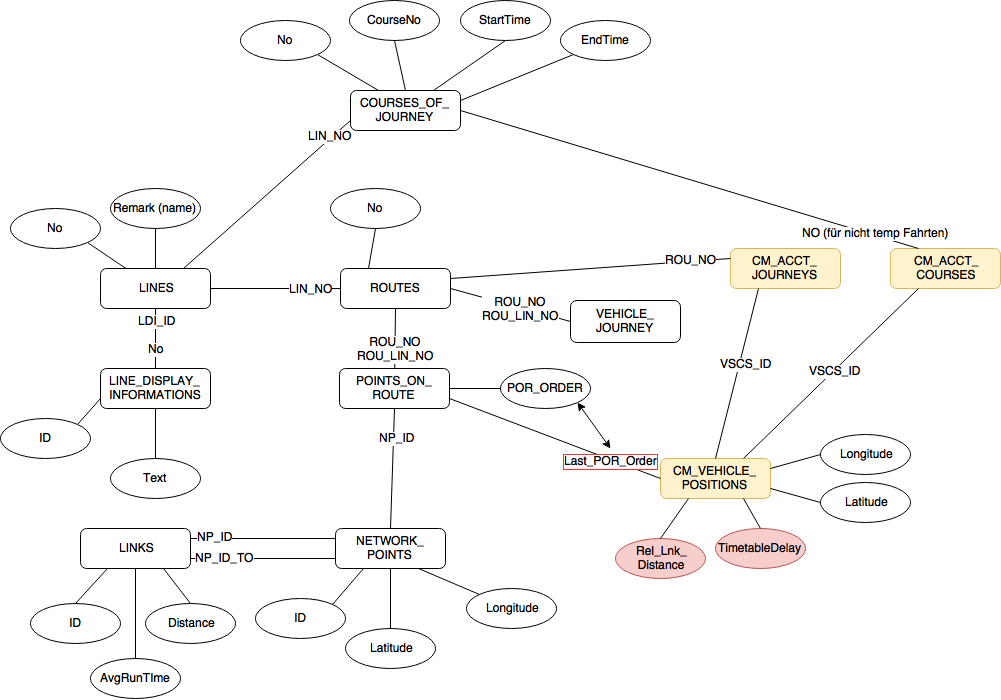
\includegraphics[width=15cm]{res/BVG-DB.png}
	\caption{Datenbank Schema aus SC05 und SC51}
	\label{img:db-bvg}
\end{figure}
 
\section{Schnittstellendefinition}

\section{genutzte Komponenten}
